\chapter{Introduction}

The field of autonomous driving agents has rapidly increased in modern car manufacturing. Current research topic rises the agents from parking or lane keeping assistant fully autonomous driving agents obeying the traffic rules and having the ability to react to the volatile environment in a reasonable way.

For that machine learning techniques have proven themselves as an essential part. But in order to fulfil the security standards and create a sophisticated agent it has to be trained on hundred-thousands of scenarios each having a large set of data attached, for example sensor and camera data.
The approach of \textit{Convolutional Neural Networks} (CNNs) have been proven to be powerful enough to handle such many training iterations with a huge number of input variables, while maintaining the large learning capacity. \cite{krizhevsky2012imagenet}

A CNN, as explained in \Cref{sec:CNN}, has a general structure, but can be altered to fit into the approach in various ways influencing the result. Therefore we introduce in \Cref{sec: Deep Learning Approaches} the three main approaches of using a CNN.

Further in \Cref{sec: DLL} we see that there is the need of specific languages for the design and implementation of such agents. Two languages will be discussed and compared based on their suitability regarding the \alexnet, stated in  \Cref{subsec: AlexNet}.

\section{Neural Networks}\label{sec: NN}

The \nns are a construct adapted from biological processes. The general construct is very simple, but the expressiveness is very high but still not fully researched.
A neural net is made out of neurons and has one very basic function:
It takes a fixed number $n \in \mathbb{N}$ of the incoming values $x_i$ and multiplies them each with a specific weight $w_i$, where $0 \le i \le n$.
Also every neuron contains a bias $b$, which is a general value subtracted from the sum, so $\sum_{i=0}^{n} (x_i \cdot w_i) -b$. 
Often one applies an activation function to fix the value between 0 and 1. Such a function would be for example the sigmoid function or the ReLu. Without such a normalizing function the change in one neuron, which is very important could be very small compared to other values, which are not so important.
\todo{better example\\}
This new value gets forwarded to the neurons of the next layer.

Those neurons are ordered in different groups often called layers, as seen in \Cref{fig: Simple NN}.
\begin{enumerate}
	\item input layer (green):\\ \label{item input layer}
		This layer gets fed with the input values of the problem, which can be for example sensor data or pixel color values.
	\item hidden layer (blue):\\\label{item hidden layer}
		The hidden layer consists of neurons receiving the values from the previous layer, while not being obliged to have the same number of neurons (c.f. \Cref{fig: Simple NN}).
		Different hidden layer architectures can be distinguished to be deep (c.f. \Cref{fig: Deep Neural Net}). This means, that there are multiple layers of neurons within the hidden layer itself.\\
		Also a variation within the hidden layer is the possibility of fully connectivity (c.f. \Cref{fig: not fullyconnected Neural Net}). Thus some neurons don't forward their value to every neuron of the next layer.\\
		There is no rule of how to construct the best hidden layer, considering number of sub-layers, neurons per layer or the connectivity.
	\item output layer (yellow):\label{item output layer}
		The output neurons contain the value the \nn produces. Depending on the \nns purpose it can be for example a confidence value of a classification, like recognizing a stop sign, or the value of changing the steering wheel angle. 
\end{enumerate}

In order to train a \nn one has to define the behaviour the \nn should have. In an image classification example one should know what the correct class of a given image of a sign is, i.e. a speed limit sign.\\
A \nn can then be trained by giving it values for the input layer and comparing the values of the output layer with the solutions it should have resulted in. The difference can then be checked. Such a difference can be simply \texttt{true}/\texttt{false} or a value indicating how big the difference is. In the example of signs a classification of a ``speed limit 70''-sign as ``speed limit 50''-sign is still wrong, but as bad as a classification as a ``stop''-sign.\\
Using this difference value the \nn can use linear algebra algorithms to adjust the weights $w_i$ and biases $b$ to improve the output iteratively.

For further information about the underlying training algorithms please see %TODO

\todo{training ref\\}
\begin{figure}
	\centering
	\tikzset{input/.style = {ellipse,draw,fill=green!50!white, initial, initial text =}}
	\tikzset{hidden/.style = {ellipse,draw,fill=blue!50!white}}
	\tikzset{output/.style = {ellipse,draw,fill=yellow!50!white}}
	\begin{subfigure}[b]{0.25\textwidth}
	\begin{tikzpicture}[node distance = .5cm, on grid,auto]		
		\node[input] (i1) {};
		\node[input, below = of i1] (i2) {};
		\node[input, below = of i2] (i3) {};
		
		\node[hidden, above right = .25cm and 1cm of i1] (h1) {};
		\node[hidden, below = of h1] (h2) {};
		\node[hidden, below = of h2] (h3) {};
		\node[hidden, below = of h3] (h4) {};
		
		\node[output , right = 1cm of h2] (o1) {};
		\node[output , below = of o1] (o2) {};
		\coordinate[right = of o1] (c1) {};
		\coordinate[right = of o2] (c2) {};
		
		\path[->] (i1.east) edge (h1.west)
					(i1.east) edge (h2.west)
					(i1.east) edge (h3.west)
					(i1.east) edge (h4.west);
		\path[->] (i2.east) edge (h1.west)
					(i2.east) edge (h2.west)
					(i2.east) edge (h3.west)
					(i2.east) edge (h4.west);
		\path[->] (i3.east) edge (h1.west)
					(i3.east) edge (h2.west)
					(i3.east) edge (h3.west)
					(i3.east) edge (h4.west);
		\path[->] (h1.east) edge (o1.west)
				  (h2.east) edge (o1.west)
				  (h3.east) edge (o1.west)
				  (h4.east) edge (o1.west);
		\path[->] (h1.east) edge (o2.west)
					(h2.east) edge (o2.west)
					(h3.east) edge (o2.west)
					(h4.east) edge (o2.west);
		\path[->] (o1) edge (c1)
				  (o2) edge (c2);		
	\end{tikzpicture}	
	\caption{}
	\label{fig: Simple NN}
	\end{subfigure}
	\begin{subfigure}[b]{0.40\textwidth}
	\begin{tikzpicture}[node distance = .5cm, on grid,auto]		
	\node[input] (i1) {};
	\node[input, below = of i1] (i2) {};
	\node[input, below = of i2] (i3) {};
	
	\node[hidden, above right = .25cm and 1cm of i1] (h11) {};
	\node[hidden, below = of h11] (h21) {};
	\node[hidden, below = of h21] (h31) {};
	\node[hidden, below = of h31] (h41) {};
	
	\node[hidden, above right = .5cm and 1cm of h11] (h12) {};
	\node[hidden, below = of h12] (h22) {};
	\node[hidden, below = of h22] (h32) {};
	\node[hidden, below = of h32] (h42) {};
	\node[hidden, below = of h42] (h52) {};
	\node[hidden, below = of h52] (h62) {};
	
	\node[right =0.5cm of h12] (d1) {\dots};
	\node[below = of d1] (d2) {\dots};
	\node[below = of d2] (d3) {\dots};
	\node[below = of d3] (d4) {\dots};
	\node[below = of d4] (d5) {\dots};
	\node[below = of d5] (d6) {\dots};
	
	\node[hidden, right = 0.5cm of d1] (h13) {};
	\node[hidden, below = of h13] (h23) {};
	\node[hidden, below = of h23] (h33) {};
	\node[hidden, below = of h33] (h43) {};
	\node[hidden, below = of h43] (h53) {};
	\node[hidden, below = of h53] (h63) {};
	
	\node[output , right = 1cm of h33] (o1) {};
	\node[output , below = of o1] (o2) {};
	\coordinate[right = of o2] (c1) {};
	\coordinate[right = of o1] (c1) {};
	
	\path[->] (i1.east) edge (h11.west)
				(i1.east) edge (h21.west)
				(i1.east) edge (h31.west)
				(i1.east) edge (h41.west);
	\path[->] (i2.east) edge (h11.west)
				(i2.east) edge (h21.west)
				(i2.east) edge (h31.west)
				(i2.east) edge (h41.west);
	\path[->] (i3.east) edge (h11.west)
				(i3.east) edge (h21.west)
				(i3.east) edge (h31.west)
				(i3.east) edge (h41.west);
	\path[->] (h11.east) edge (h12.west)			
				(h11.east) edge (h22.west)
				(h11.east) edge (h32.west)
				(h11.east) edge (h42.west)
				(h11.east) edge (h52.west)
				(h11.east) edge (h62.west);
	\path[->] (h21.east) edge (h12.west)			
				(h21.east) edge (h22.west)
				(h21.east) edge (h32.west)
				(h21.east) edge (h42.west)
				(h21.east) edge (h52.west)
				(h21.east) edge (h62.west);
	\path[->] (h31.east) edge (h12.west)			
				(h31.east) edge (h22.west)
				(h31.east) edge (h32.west)
				(h31.east) edge (h42.west)
				(h31.east) edge (h52.west)
				(h31.east) edge (h62.west);			
	\path[->] (h41.east) edge (h12.west)			
				(h41.east) edge (h22.west)
				(h41.east) edge (h32.west)
				(h41.east) edge (h42.west)
				(h41.east) edge (h52.west)
				(h41.east) edge (h62.west);
					
	\path[->] (h13.east) edge (o1.west)
				(h23.east) edge (o1.west)
				(h33.east) edge (o1.west)
				(h43.east) edge (o1.west)
				(h53.east) edge (o1.west)
				(h63.east) edge (o1.west);		
	\path[->] (h13.east) edge (o2.west)
				(h23.east) edge (o2.west)
				(h33.east) edge (o2.west)
				(h43.east) edge (o2.west)
				(h53.east) edge (o2.west)
				(h63.east) edge (o2.west);		
	\end{tikzpicture}
	\caption{}
	\label{fig: Deep Neural Net}
	\end{subfigure}	
	\begin{subfigure}[b]{0.32\textwidth}
		\begin{tikzpicture}[node distance = .5cm, on grid,auto]		
		\node[input] (i1) {};
		\node[input, below = of i1] (i2) {};
		\node[input, below = of i2] (i3) {};
		
		\node[hidden, above right = .25cm and 1cm of i1] (h11) {};
		\node[hidden, below = of h11] (h21) {};
		\node[hidden, below = of h21] (h31) {};
		\node[hidden, below = of h31] (h41) {};
		
		\node[hidden, above right = .5cm and 1cm of h11] (h12) {};
		\node[hidden, below = of h12] (h22) {};
		\node[hidden, below = of h22] (h32) {};
		\node[hidden, below = of h32] (h42) {};
		\node[hidden, below = of h42] (h52) {};
		\node[hidden, below = of h52] (h62) {};
		
		
		\node[output , right = 1cm of h32] (o1) {};
		\node[output , below = of o1] (o2) {};
		\coordinate[right = of o2] (c1) {};
		\coordinate[right = of o1] (c1) {};
		
		\path[->] (i1.east) edge (h11.west)
			(i1.east) edge (h21.west)
			(i1.east) edge (h31.west)
			(i1.east) edge (h41.west);
		\path[->] (i2.east) edge (h11.west)
			(i2.east) edge (h21.west)
			(i2.east) edge (h31.west)
			(i2.east) edge (h41.west);
		\path[->] (i3.east) edge (h11.west)
			(i3.east) edge (h21.west)
			(i3.east) edge (h41.west);

		\path[->] (h11.east) edge (h12.west)			
			(h11.east) edge (h22.west)
			(h11.east) edge (h32.west);
		\path[->] (h21.east) edge (h22.west)
			(h21.east) edge (h32.west)
			(h21.east) edge (h42.west)
			(h21.east) edge (h12.west);
		\path[->] (h31.east) edge (h32.west)
			(h31.east) edge (h42.west)
			(h31.east) edge (h52.west)
			(h31.east) edge (h62.west);			
		\path[->] (h41.east) edge (h42.west)
			(h41.east) edge (h52.west)
			(h41.east) edge (h62.west);
		\path[->] (h12.east) edge (o1.west)
			(h22.east) edge (o1.west)
			(h52.east) edge (o1.west)
			(h62.east) edge (o1.west);		
		\path[->] (h12.east) edge (o2.west)
			(h22.east) edge (o2.west)
			(h32.east) edge (o2.west)
			(h42.east) edge (o2.west)
			(h52.east) edge (o2.west)
			(h62.east) edge (o2.west);		
		\end{tikzpicture}
		\caption{}
		\label{fig: not fullyconnected Neural Net}
	\end{subfigure}
	% das Dritte ist wenig Sinvoll vom Aufbau her
\end{figure}


\section{Convolutional Neural Network (CNN)}\label{sec:CNN}

A CNN is a special class of deep feed-forward \nns. On of the main design goals of a CNN is that they require a minimal amount of preprocessing. This is an important aspect, because they are often fed with images. Preprocessing high resolution images is very costly in terms of computational time. In the context of autonomous driving the time is even more crucial, since the driving agent needs to be able to react to spontaneous events.

Like most parts of \nns, also the CNNs are inspired by biological processes. It is mainly based on the connectivity pattern of an animals visual cortex, where special neurons respond only to stimuli of their receptive field, represented as rectangles lying in the image. Partially overlapping guarantees a complete coverage of the field of view. \cite{wiki:CNN}

The partitioning into those rectangles also has the advantage, that the size of the input image is not relevant. If there would be a direct correspondence of a pixel to one input value then a change of the size would infer null values or additional input values, where the weights are not directly well suited. But with partitioning it into sub-rectangles of the image the values can be unified by selecting these rectangles relative to the size. %TODO ref

These separation into those receptive fields has also the advantage that is reduces the effort to train a CNN. The weights and biases of neurons of each receptive field are equal. This is reasonable since for example a speed limit road sign should be identified independent whether it is located next to the road, like on a normal road, or above the road, like on an highway. %TODO: ref

Further CNNs make strong and mostly correct assumptions about the nature of images, like stationary of statistics and locality of pixel dependencies. This leads to fewer connections and parameters, compared to a normal feed-forward neural net with similar sized layers, and therefore reduces the time it takes to be trained, while being only slightly worse in their best-performance. \cite{krizhevsky2012imagenet}

\todo{ erklären von kernel/filter\\}

\subsection{AlexNet} \label{subsec: AlexNet}

The \textit{\alexnet} is on of the best performing CNN architectures currently known. It is trained on the ImageNet subsets of \texttt{ILSVRC-2010} and \texttt{ILSVRC-2012}\footnote{Further information: http://www.image-net.org/challenges/LSVRC/} and became famous because of its result being way ahead of all other competitors.

A highly optimized GPU implementation of this architecture combined with innovative features is publicly available. Those features lead to improve performance and reduce training time.
An important note is that the original test is dated back to 2012 and therefore was used with an overall GPU memory of 6GB, with which training took abound six days. With modern hardware the training can be done faster, or the model can be trained much more. \cite{krizhevsky2012imagenet}

\todo{maybe calc the possible speed up based on ``Hardware for Machine Learning''}

\begin{figure}[ht]
	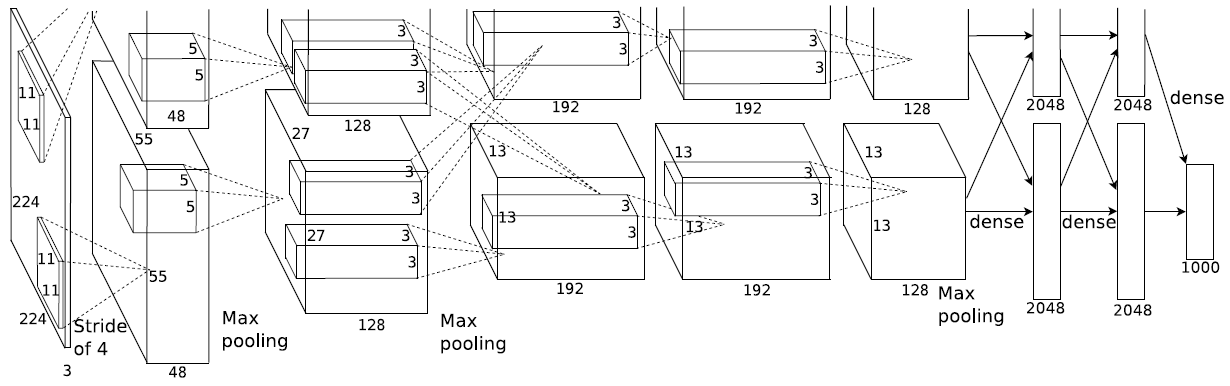
\includegraphics[scale = 0.5]{src/pic/AlexNet-structure.PNG}
	\caption{The \alexnet-architecture for two GPUs. It consists of 5 convolutional layers (at the beginning) and three fully-connected layers (at the end). The GPUs only communicate between two layers, but never within a layer.\cite{krizhevsky2012imagenet}}
	\label{pic: AlexNet}
	\todo{Vereinfachen der Zeichnung\\}
\end{figure}

\section{Available Deep Learning Approaches}\label{sec: Deep Learning Approaches}

There are various approaches of autonomous driving agents making a variety of assumptions and differ in numerous options. But they can be mostly categorized into two major groups of approaches: mediated perception approaches and behavior reflex approaches. \cite{chen2015deepdriving}

In this paper we further analyze a suggested third group, called direct perception, which can traced to \cite{gibson1979ecological} in the mid 50's, but was sharply criticized by researchers of the other two groups, i.e. in \cite{ullman1980against}. %TODO: fix 60's to be the first

All these three groups differ in the way of interpreting the given sensor data and whether or not to create a some what bigger picture based on consequent data.

\subsection{Mediated Perception} \label{subsec: Mediated Perception}

The mediated perception approach is a multi-component continuous process. Every component recognizes specific aspects for driving. For example traffic signs, lanes, other cars. Those components are then combined into one single world state representing the cars surrounding based on the sensor data. \cite{KITTI}\\
These world states are 3D models of the current world. Cars are identified using a classifier and then often surrounded by a 3D bounding box. An example can be seen in \Cref{pic: 3D Bounding Box}. By comparing different frames generated one can estimate the speed and distance to those objects and derive an A.I. based precedence behavior. \cite{KITTI}\cite{chen2015deepdriving}

The often stated problems with such approaches are, that computing such a scene is costly in terms of computation time. Some information is irrelevant, redundant or even misleading due to inaccuracy of sensors. To perform a right turn the sensor information of the distance to a car left behind me is irrelevant, but becomes very important when taking a left turn.\\
Additionally many of the subtasks are still open research topics themselves. For example a reliable lane detection throughout various weather conditions or even a new road not having any drawn lines yet. \cite{aly2008real}\\
Also mediated perception approaches require very detailed information up front, like up-to-date maps.

The approach of mediated perception is a reasonable and very sturdy way of handling such a complex task, but has its drawbacks regarding computational time and additional knowledge.

\begin{figure}
	\centering
	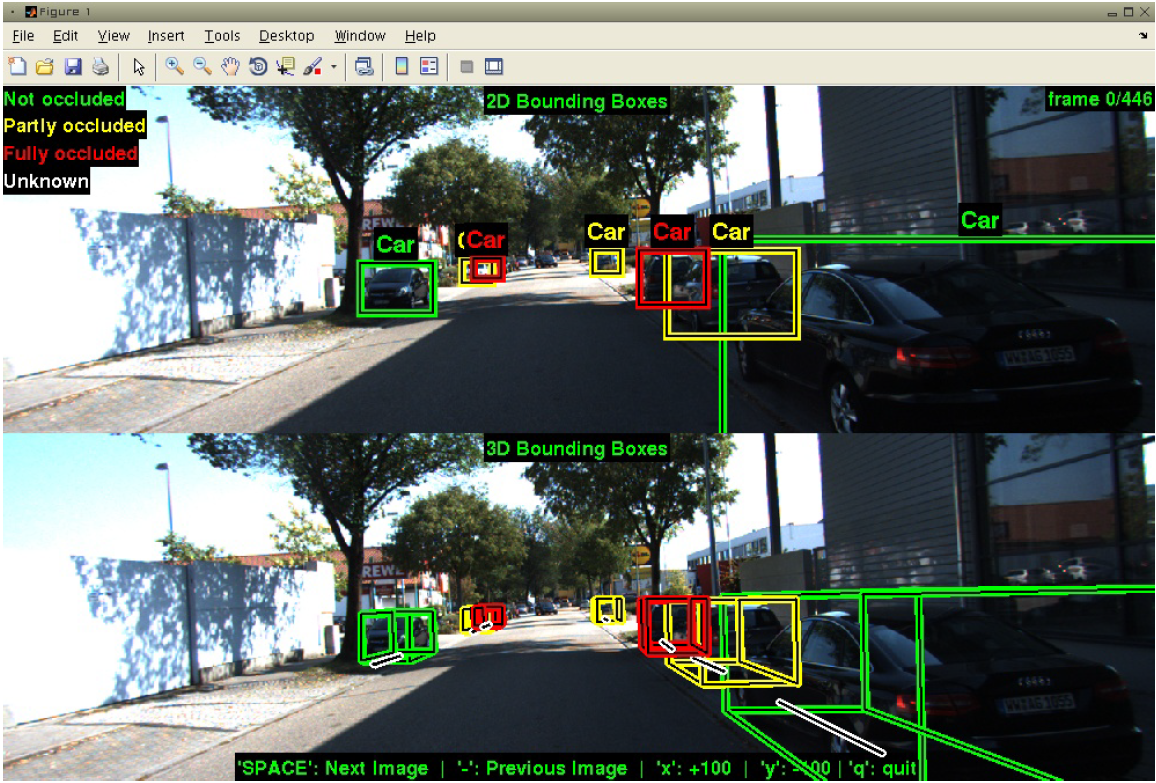
\includegraphics[scale=0.4]{src/pic/3D-boundingbox-example.png}
	\caption{An example of a scene using 3D bounding boxes. This image is taken from the MATLAB delvopment kit of \cite{KITTI}}
	\label{pic: 3D Bounding Box}
\end{figure}

\subsection{Behavior Reflex}\label{subsec: Behavior Reflex}

The behavior reflex approach of constructing a reliable autonomous driving agent can be dated back to 1989 , where researchers tried to directly map a single frame to a decision of a steering angle. For such approaches a quite simple \nn were created. \\
The network \alvinn, shown in \Cref{pic: ALVINN}, consisted of a single hidden layer, used back-propagation and is fed by two cameras: a $30\times32$ pixel video and a $8\times32$ pixel range finder retina. The input neurons fired depending on the blue color band of its pixel, because it is believed to infer the highest contrast between road and non-road. The difference in color of road and non-road was fed back to the network. The bias (activation level) is proportional to the proximity of the corresponding area, based on the likelihood and importance of having road in particular fields of the image.\cite{pomerleau1989alvinn}\\
For example having recognized that the road abruptly ends right in front of the car is more important than recognizing that there is a road in the top left corner.\\

Such systems, even though they are simple compared to the in \Cref{subsec: Mediated Perception} mentioned mediated perception approaches, have been proven to have the capability to perform simple tasks. It can elegantly be trained by having a human drive a car with the cameras equipped and forward the images to the \nn and adding the current steering angles as a label.\cite{chen2015deepdriving}\\

The problem with behavior reflex approaches is, that they reach their limits very early when adding more complex scenarios. Having simple alternations to the trained scenarios, which enforce a different behavior, is very hard to train to such a \nn.\\
For example comparing a simple straight 3 lane road with the car in the middle, as sketched in \Cref{fig: behavior sketches}. The system is confidently able to hold the angle and make small adjustments to stay in the lane (\Cref{fig: behavior sketches: free lane}). But what if on the same road there is an other car in the middle lane in front of the agent, which is slower? Having quite the same input the system would have to overtake the car left or right (considering an american highway) (\Cref{fig: behavior sketches: blocked lane}). Now also considering a car in front, which has the same speed. One can simple stay in the lane (\Cref{fig: behavior sketches: shared lane}). This maneuver is very hard to train to a simple \nn like \alvinn.

\todo{noch mehr?\\}

\begin{figure}
	\centering	
	\tikzset{->,very thick,>=stealth}
	\begin{subfigure}[b]{0.32\textwidth}
		\begin{tikzpicture}[scale=0.9] % left picture
		\newcommand{\lineLength}{0.75}
		\newcommand{\lineSpace}{0.5}
		\newcommand{\startSpace}{0.25}
		
		\fill[green!50!black] (0,0) rectangle (5,5);		% background
		\fill[gray!50!black] (0.5,0) rectangle (4.5,5);     % pavement
		\fill[yellow!75!black] (0.55,0) rectangle (0.6,5);  % left yellow line
		\fill[yellow!75!black] (4.4,0) rectangle (4.45,5);  % right yellow line
		
		% left lane breaks		
		\fill[white] (1.84,\startSpace) rectangle (1.86,\lineLength+\startSpace);		
		\fill[white] (1.84,1*\lineLength + 1*\lineSpace + \startSpace) rectangle (1.86,2*\lineLength + 1*\lineSpace + \startSpace);
		\fill[white] (1.84,2*\lineLength + 2*\lineSpace + \startSpace) rectangle (1.86,3*\lineLength + 2*\lineSpace + \startSpace);
		\fill[white] (1.84,3*\lineLength + 3*\lineSpace + \startSpace) rectangle (1.86,4*\lineLength + 3*\lineSpace + \startSpace);
		
		% right line breaks
		\fill[white] (3.12,\startSpace) rectangle (3.14,\lineLength+\startSpace);		
		\fill[white] (3.12,1*\lineLength + 1*\lineSpace + \startSpace) rectangle (3.14,2*\lineLength + 1*\lineSpace + \startSpace);
		\fill[white] (3.12,2*\lineLength + 2*\lineSpace + \startSpace) rectangle (3.14,3*\lineLength + 2*\lineSpace + \startSpace);
		\fill[white] (3.12,3*\lineLength + 3*\lineSpace + \startSpace) rectangle (3.14,4*\lineLength + 3*\lineSpace + \startSpace);
		
		% cars
		\fill[red] (2.1,0.2) rectangle (2.1 + 0.8,0.2 + 1.5);
		\draw[->,very thick,  color = white] (2.5,0.4) -- (2.5,1.5);
		\draw[->,very thick,  color = green!75!black] (2.5,2) -- (2.5,3);
		
		%		\node [trapezium, minimum width = 3.6cm, trapezium angle=25,rotate = 180, opacity = 0.4, color = gray!50!white, fill] at (2.5,2) (test) {};
		%		\fill[gray!50!white, opacity = 0.4] (0.5,2.378) rectangle (4.5,5);
		\end{tikzpicture}
		\caption{free lane}
		\label{fig: behavior sketches: free lane}
	\end{subfigure}
	\begin{subfigure}[b]{0.32\textwidth}
		\begin{tikzpicture}[scale=0.9] % middle picture
		\newcommand{\lineLength}{0.75}
		\newcommand{\lineSpace}{0.5}
		\newcommand{\startSpace}{0.25}
		
		\fill[green!50!black] (0,0) rectangle (5,5);		% background
		\fill[gray!50!black] (0.5,0) rectangle (4.5,5);     % pavement
		\fill[yellow!75!black] (0.55,0) rectangle (0.6,5);  % left yellow line
		\fill[yellow!75!black] (4.4,0) rectangle (4.45,5);  % right yellow line
		
		% left lane breaks		
		\fill[white] (1.84,\startSpace) rectangle (1.86,\lineLength+\startSpace);		
		\fill[white] (1.84,1*\lineLength + 1*\lineSpace + \startSpace) rectangle (1.86,2*\lineLength + 1*\lineSpace + \startSpace);
		\fill[white] (1.84,2*\lineLength + 2*\lineSpace + \startSpace) rectangle (1.86,3*\lineLength + 2*\lineSpace + \startSpace);
		\fill[white] (1.84,3*\lineLength + 3*\lineSpace + \startSpace) rectangle (1.86,4*\lineLength + 3*\lineSpace + \startSpace);
		
		% right line breaks
		\fill[white] (3.12,\startSpace) rectangle (3.14,\lineLength+\startSpace);		
		\fill[white] (3.12,1*\lineLength + 1*\lineSpace + \startSpace) rectangle (3.14,2*\lineLength + 1*\lineSpace + \startSpace);
		\fill[white] (3.12,2*\lineLength + 2*\lineSpace + \startSpace) rectangle (3.14,3*\lineLength + 2*\lineSpace + \startSpace);
		\fill[white] (3.12,3*\lineLength + 3*\lineSpace + \startSpace) rectangle (3.14,4*\lineLength + 3*\lineSpace + \startSpace);
		
		% cars
		\fill[red] (2.1,0.2) rectangle (2.1 + 0.8,0.2 + 1.5);	% agent
		\draw[->,very thick,  color = white] (2.5,0.4) -- (2.5,1.5);
		\draw[->,very thick,  color = green!75!black] (2,1.8) -- (1.3,2.5) -- (1.3,3);
		\draw[->,very thick,  color = green!75!black] (3,1.8) -- (3.8,2.5) -- (3.8,3);
		
		
		\fill[orange] (2.1,3.2) rectangle (2.1 + 0.8,3.2 + 1.5);	% other car
		\draw[->,very thick,  color = white] (2.5,3.4) -- (2.5,4);
		\end{tikzpicture}
		\caption{slower car in the same lane}
		\label{fig: behavior sketches: blocked lane}
	\end{subfigure}
	\begin{subfigure}[b]{0.32\textwidth}
		\begin{tikzpicture}[scale=0.9] % right picture
		\newcommand{\lineLength}{0.75}
		\newcommand{\lineSpace}{0.5}
		\newcommand{\startSpace}{0.25}
		
		\fill[green!50!black] (0,0) rectangle (5,5);		% background
		\fill[gray!50!black] (0.5,0) rectangle (4.5,5);     % pavement
		\fill[yellow!75!black] (0.55,0) rectangle (0.6,5);  % left yellow line
		\fill[yellow!75!black] (4.4,0) rectangle (4.45,5);  % right yellow line
		
		% left lane breaks		
		\fill[white] (1.84,\startSpace) rectangle (1.86,\lineLength+\startSpace);		
		\fill[white] (1.84,1*\lineLength + 1*\lineSpace + \startSpace) rectangle (1.86,2*\lineLength + 1*\lineSpace + \startSpace);
		\fill[white] (1.84,2*\lineLength + 2*\lineSpace + \startSpace) rectangle (1.86,3*\lineLength + 2*\lineSpace + \startSpace);
		\fill[white] (1.84,3*\lineLength + 3*\lineSpace + \startSpace) rectangle (1.86,4*\lineLength + 3*\lineSpace + \startSpace);
		
		% right line breaks
		\fill[white] (3.12,\startSpace) rectangle (3.14,\lineLength+\startSpace);		
		\fill[white] (3.12,1*\lineLength + 1*\lineSpace + \startSpace) rectangle (3.14,2*\lineLength + 1*\lineSpace + \startSpace);
		\fill[white] (3.12,2*\lineLength + 2*\lineSpace + \startSpace) rectangle (3.14,3*\lineLength + 2*\lineSpace + \startSpace);
		\fill[white] (3.12,3*\lineLength + 3*\lineSpace + \startSpace) rectangle (3.14,4*\lineLength + 3*\lineSpace + \startSpace);
		
		% cars
		\fill[red] (2.1,0.2) rectangle (2.1 + 0.8,0.2 + 1.5);
		\draw[->,very thick,  color = white] (2.5,0.4) -- (2.5,1.5);
		\draw[->,very thick,  color = green!75!black] (2.5,2) -- (2.5,3);
		
		\fill[orange] (2.1,3.2) rectangle (2.1 + 0.8,3.2 + 1.5);	% other car
		\draw[->,very thick,  color = white] (2.5,3.4) -- (2.5,4.5);
		\end{tikzpicture}
		\caption{equal fast car in same lane}
		\label{fig: behavior sketches: shared lane}
	\end{subfigure}
	\caption{The 3 scenarios causing problems with behavior reflex approaches. The red block is the agent, the orange block the other car, the white arrows indicate the velocity and the green arrows the logically deduced behaviors.}
	\label{fig: problematic behavior sketches}
\end{figure}

\begin{figure}
	\centering
	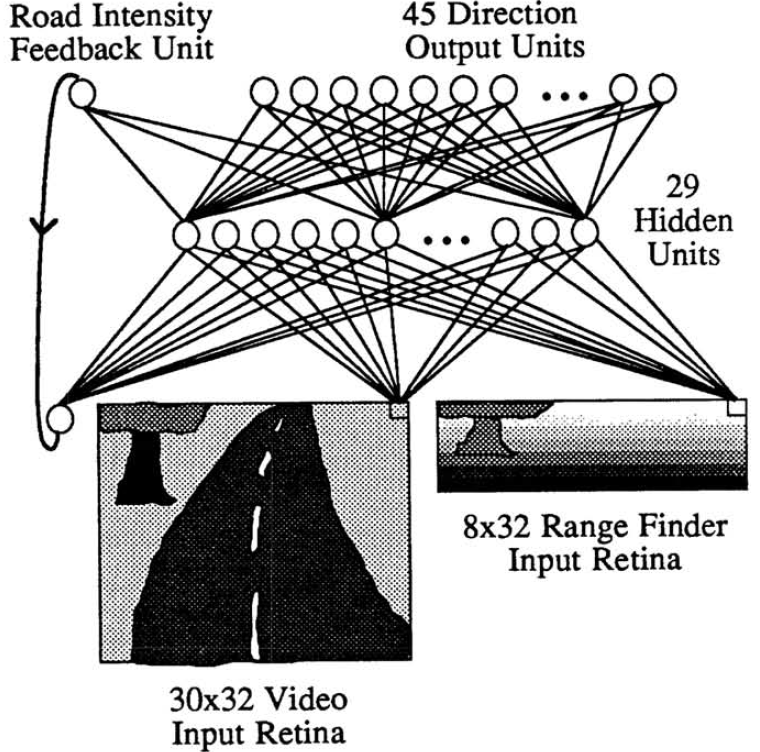
\includegraphics[scale=0.4]{src/pic/ALVINN.png}
	\caption{The \nn called \alvinn and used as a behavior reflex based autonomous agent. \cite{pomerleau1989alvinn}}
	\label{pic: ALVINN}
\end{figure}

\subsection{Direct Perception}\label{subsec: Direct Perception}

%In this paper we further analyze a suggested third group, called direct perception, which can traced to \cite{gibson2014ecological} in the late 80's, but was sharply criticized by researchers of the other two groups, i.e. in \cite{ullman1980against}.

The direct perception is the third group of approaches, which can be dated back to the 1954 and was initially mainly researched by James J. Gibson. \cite{gibson1954theory} The approach is based on analyzing a picture not simply deducing a steering angle, or velocity change, like the behavior reflex approaches (cf. \Cref{subsec: Behavior Reflex}), but also performing further computation without parsing it into a 3D world state model like the mediated perception approaches (cf. \Cref{subsec: Mediated Perception}). \cite{chen2015deepdriving}\\
So it is a third paradigm, which can be interpreted as a hybrid of the two other paradigms. The approach tries to identify only the meaningful affordance indicators and make a decision based on those parameters. 

We further consider a design based on \cite{chen2015deepdriving} and their way of training.

The original paper \cite{chen2015deepdriving} stated the a total number of 13 indicators separated in two states to be sufficient. The states are: in line driving (following the lane) and on line driving (changing lanes). The values themselves can be categorized as: preceding car distances, distances to the lane markers and the steering angle. The indicators and their affiliation to the states can be seen in \Cref{lst: affordance indicators}.

\begin{figure}
\centering
\todoLine
\begin{lstlisting}
always:
  1) angle: angle between the car's heading and the tangent of the road
"in lane system", when driving in the lane:
  2) toMarking LL: distance to the left lane marking of the left lane
  3) toMarking ML: distance to the left lane marking of the current lane
  4) toMarking MR: distance to the right lane marking of the current lane
  5) toMarking RR: distance to the right lane marking of the right lane
  6) dist LL: distance to the preceding car in the left lane
  7) dist MM: distance to the preceding car in the current lane
  8) dist RR: distance to the preceding car in the right lane
"on marking system", when driving on the lane marking:
  9) toMarking L: distance to the left lane marking
  10) toMarking M: distance to the central lane marking
  11) toMarking R: distance to the right lane marking
  12) dist L: distance to the preceding car in the left lane
  13) dist R: distance to the preceding car in the right lane
\end{lstlisting}
\todoLine
\caption{The affordance indicators and their affiliation states}
\label{lst: affordance indicators}
\end{figure}

Based on the current state, all affordance indicators of the other state are not used, since the other state is defined to be inactive.\\
In order to identify the current state the host car is in, every state has their respective region, where they are active with an overlapping region for smooth transitioning.

%These affordance values and their recognition in an image is trained to the \nn.

\begin{figure}
	\centering	
	\tikzset{->,very thick,>=stealth}
	\begin{subfigure}[b]{0.32\textwidth}
		\begin{tikzpicture}[scale=0.9] % top left picture
		\newcommand{\lineLength}{0.75}
		\newcommand{\lineSpace}{0.5}
		\newcommand{\startSpace}{0.25}
		
		\fill[green!50!black] (0,0) rectangle (5,5);		% background
		\fill[gray!50!black] (0.5,0) rectangle (4.5,5);     % pavement
		\fill[yellow!75!black] (0.55,0) rectangle (0.6,5);  % left yellow line
		\fill[yellow!75!black] (4.4,0) rectangle (4.45,5);  % right yellow line
		
		% left lane breaks		
		\fill[white] (1.84,\startSpace) rectangle (1.86,\lineLength+\startSpace);		
		\fill[white] (1.84,1*\lineLength + 1*\lineSpace + \startSpace) rectangle (1.86,2*\lineLength + 1*\lineSpace + \startSpace);
		\fill[white] (1.84,2*\lineLength + 2*\lineSpace + \startSpace) rectangle (1.86,3*\lineLength + 2*\lineSpace + \startSpace);
		\fill[white] (1.84,3*\lineLength + 3*\lineSpace + \startSpace) rectangle (1.86,4*\lineLength + 3*\lineSpace + \startSpace);
		
		% right line breaks
		\fill[white] (3.12,\startSpace) rectangle (3.14,\lineLength+\startSpace);		
		\fill[white] (3.12,1*\lineLength + 1*\lineSpace + \startSpace) rectangle (3.14,2*\lineLength + 1*\lineSpace + \startSpace);
		\fill[white] (3.12,2*\lineLength + 2*\lineSpace + \startSpace) rectangle (3.14,3*\lineLength + 2*\lineSpace + \startSpace);
		\fill[white] (3.12,3*\lineLength + 3*\lineSpace + \startSpace) rectangle (3.14,4*\lineLength + 3*\lineSpace + \startSpace);
		
		% cars
		\fill[red] (2.1,0.2) rectangle (2.1 + 0.8,0.2 + 1.5);	% agent		
		\fill[orange] (0.8,3.9) rectangle (0.8 + 0.8,3.9 + 1.1);	% left other car
		\fill[orange] (2.1,2.6) rectangle (2.1 + 0.8,2.6 + 1.5);	% middle other car
		\fill[orange] (3.4,3.2) rectangle (3.4 + 0.8,3.2 + 1.5);	% right other car
		\end{tikzpicture}
		\caption{slower car in the same lane}
		\label{fig: affordance indicators: in lane - lines}
	\end{subfigure}
	\begin{subfigure}[b]{0.32\textwidth}
		\begin{tikzpicture}[scale=0.9] % top middles picture
		\newcommand{\lineLength}{0.75}
		\newcommand{\lineSpace}{0.5}
		\newcommand{\startSpace}{0.25}
		
		\fill[green!50!black] (0,0) rectangle (5,5);		% background
		\fill[gray!50!black] (0.5,0) rectangle (4.5,5);     % pavement
		\fill[yellow!75!black] (0.55,0) rectangle (0.6,5);  % left yellow line
		\fill[yellow!75!black] (4.4,0) rectangle (4.45,5);  % right yellow line
		
		% left lane breaks		
		\fill[white] (1.84,\startSpace) rectangle (1.86,\lineLength+\startSpace);		
		\fill[white] (1.84,1*\lineLength + 1*\lineSpace + \startSpace) rectangle (1.86,2*\lineLength + 1*\lineSpace + \startSpace);
		\fill[white] (1.84,2*\lineLength + 2*\lineSpace + \startSpace) rectangle (1.86,3*\lineLength + 2*\lineSpace + \startSpace);
		\fill[white] (1.84,3*\lineLength + 3*\lineSpace + \startSpace) rectangle (1.86,4*\lineLength + 3*\lineSpace + \startSpace);
		
		% right line breaks
		\fill[white] (3.12,\startSpace) rectangle (3.14,\lineLength+\startSpace);		
		\fill[white] (3.12,1*\lineLength + 1*\lineSpace + \startSpace) rectangle (3.14,2*\lineLength + 1*\lineSpace + \startSpace);
		\fill[white] (3.12,2*\lineLength + 2*\lineSpace + \startSpace) rectangle (3.14,3*\lineLength + 2*\lineSpace + \startSpace);
		\fill[white] (3.12,3*\lineLength + 3*\lineSpace + \startSpace) rectangle (3.14,4*\lineLength + 3*\lineSpace + \startSpace);
		
		% cars
		\fill[red] (2.1,0.2) rectangle (2.1 + 0.8,0.2 + 1.5);
		\fill[orange] (0.8,3.9) rectangle (0.8 + 0.8,3.9 + 1.1);	% left other car
		\fill[orange] (2.1,2.6) rectangle (2.1 + 0.8,2.6 + 1.5);	% middle other car
		\fill[orange] (3.4,3.2) rectangle (3.4 + 0.8,3.2 + 1.5);	% right other car
		\end{tikzpicture}
		\caption{equal fast car in same lane}
		\label{fig: affordance indicators: in lane - cars}
	\end{subfigure}
	\begin{subfigure}[b]{0.32\textwidth}
		\begin{tikzpicture}[scale=0.9] % top left picture
		\newcommand{\lineLength}{0.75}
		\newcommand{\lineSpace}{0.5}
		\newcommand{\startSpace}{0.25}
		
		\fill[green!50!black] (0,0) rectangle (5,5);		% background
		
%		\draw [-,gray!50!black,thick,domain=0:60] plot ({2.5*cos(\x)-1.25}, {2.5*sin(\x)});
%		\draw [-,gray!50!black,thick,domain=16:50] plot ({6.5*cos(\x)-1.25}, {6.5*sin(\x)});
%		\fill[gray!50!black] (0.5,0) rectangle (4.5,5);     % pavement
		
%		\fill[yellow!75!black] (0.55,0) rectangle (0.6,5);  % left yellow line
%		\fill[yellow!75!black] (4.4,0) rectangle (4.45,5);  % right yellow line
		
		% left lane breaks		
%		\fill[white] (1.84,\startSpace) rectangle (1.86,\lineLength+\startSpace);		
%		\fill[white] (1.84,1*\lineLength + 1*\lineSpace + \startSpace) rectangle (1.86,2*\lineLength + 1*\lineSpace + \startSpace);
%		\fill[white] (1.84,2*\lineLength + 2*\lineSpace + \startSpace) rectangle (1.86,3*\lineLength + 2*\lineSpace + \startSpace);
%		\fill[white] (1.84,3*\lineLength + 3*\lineSpace + \startSpace) rectangle (1.86,4*\lineLength + 3*\lineSpace + \startSpace);
		
		% right line breaks
%		\fill[white] (3.12,\startSpace) rectangle (3.14,\lineLength+\startSpace);		
%		\fill[white] (3.12,1*\lineLength + 1*\lineSpace + \startSpace) rectangle (3.14,2*\lineLength + 1*\lineSpace + \startSpace);
%		\fill[white] (3.12,2*\lineLength + 2*\lineSpace + \startSpace) rectangle (3.14,3*\lineLength + 2*\lineSpace + \startSpace);
%		\fill[white] (3.12,3*\lineLength + 3*\lineSpace + \startSpace) rectangle (3.14,4*\lineLength + 3*\lineSpace + \startSpace);
		
		% cars
%		\fill[red] (2.1,0.2) rectangle (2.1 + 0.8,0.2 + 1.5);
		
		%		\node [trapezium, minimum width = 3.6cm, trapezium angle=25,rotate = 180, opacity = 0.4, color = gray!50!white, fill] at (2.5,2) (test) {};
		%		\fill[gray!50!white, opacity = 0.4] (0.5,2.378) rectangle (4.5,5);
		\end{tikzpicture}
		\caption{}
		\label{fig: affordance indicators: angle}
	\end{subfigure}
	
	\begin{subfigure}[b]{0.32\textwidth}
		\begin{tikzpicture}[scale=0.9] % bottom left picture
		\newcommand{\lineLength}{0.75}
		\newcommand{\lineSpace}{0.5}
		\newcommand{\startSpace}{0.25}
		
		\fill[green!50!black] (0,0) rectangle (5,5);		% background
		\fill[gray!50!black] (0.5,0) rectangle (4.5,5);     % pavement
		\fill[yellow!75!black] (0.55,0) rectangle (0.6,5);  % left yellow line
		\fill[yellow!75!black] (4.4,0) rectangle (4.45,5);  % right yellow line
		
		% left lane breaks		
		\fill[white] (1.84,\startSpace) rectangle (1.86,\lineLength+\startSpace);		
		\fill[white] (1.84,1*\lineLength + 1*\lineSpace + \startSpace) rectangle (1.86,2*\lineLength + 1*\lineSpace + \startSpace);
		\fill[white] (1.84,2*\lineLength + 2*\lineSpace + \startSpace) rectangle (1.86,3*\lineLength + 2*\lineSpace + \startSpace);
		\fill[white] (1.84,3*\lineLength + 3*\lineSpace + \startSpace) rectangle (1.86,4*\lineLength + 3*\lineSpace + \startSpace);
		
		% right line breaks
		\fill[white] (3.12,\startSpace) rectangle (3.14,\lineLength+\startSpace);		
		\fill[white] (3.12,1*\lineLength + 1*\lineSpace + \startSpace) rectangle (3.14,2*\lineLength + 1*\lineSpace + \startSpace);
		\fill[white] (3.12,2*\lineLength + 2*\lineSpace + \startSpace) rectangle (3.14,3*\lineLength + 2*\lineSpace + \startSpace);
		\fill[white] (3.12,3*\lineLength + 3*\lineSpace + \startSpace) rectangle (3.14,4*\lineLength + 3*\lineSpace + \startSpace);
		
		% cars
		\fill[red] (1.5,0.2) rectangle (1.5 + 0.8,0.2 + 1.5);
		\fill[orange] (0.8,3.9) rectangle (0.8 + 0.8,3.9 + 1.1);	% left other car
		\fill[orange] (2.1,2.6) rectangle (2.1 + 0.8,2.6 + 1.5);	% middle other car
		\fill[gray!50!white] (3.4,3.2) rectangle (3.4 + 0.8,3.2 + 1.5);	% right other car
		%		\node [trapezium, minimum width = 3.6cm, trapezium angle=25,rotate = 180, opacity = 0.4, color = gray!50!white, fill] at (2.5,2) (test) {};
		%		\fill[gray!50!white, opacity = 0.4] (0.5,2.378) rectangle (4.5,5);
		\end{tikzpicture}
		\caption{free lane}
		\label{fig: affordance indicators: on lane - lines}
	\end{subfigure}
	\begin{subfigure}[b]{0.32\textwidth}
		\begin{tikzpicture}[scale=0.9] % bottom middle picture
		\newcommand{\lineLength}{0.75}
		\newcommand{\lineSpace}{0.5}
		\newcommand{\startSpace}{0.25}
		
		\fill[green!50!black] (0,0) rectangle (5,5);		% background
		\fill[gray!50!black] (0.5,0) rectangle (4.5,5);     % pavement
		\fill[yellow!75!black] (0.55,0) rectangle (0.6,5);  % left yellow line
		\fill[yellow!75!black] (4.4,0) rectangle (4.45,5);  % right yellow line
		
		% left lane breaks		
		\fill[white] (1.84,\startSpace) rectangle (1.86,\lineLength+\startSpace);		
		\fill[white] (1.84,1*\lineLength + 1*\lineSpace + \startSpace) rectangle (1.86,2*\lineLength + 1*\lineSpace + \startSpace);
		\fill[white] (1.84,2*\lineLength + 2*\lineSpace + \startSpace) rectangle (1.86,3*\lineLength + 2*\lineSpace + \startSpace);
		\fill[white] (1.84,3*\lineLength + 3*\lineSpace + \startSpace) rectangle (1.86,4*\lineLength + 3*\lineSpace + \startSpace);
		
		% right line breaks
		\fill[white] (3.12,\startSpace) rectangle (3.14,\lineLength+\startSpace);		
		\fill[white] (3.12,1*\lineLength + 1*\lineSpace + \startSpace) rectangle (3.14,2*\lineLength + 1*\lineSpace + \startSpace);
		\fill[white] (3.12,2*\lineLength + 2*\lineSpace + \startSpace) rectangle (3.14,3*\lineLength + 2*\lineSpace + \startSpace);
		\fill[white] (3.12,3*\lineLength + 3*\lineSpace + \startSpace) rectangle (3.14,4*\lineLength + 3*\lineSpace + \startSpace);
		
		% cars
		\fill[red] (1.5,0.2) rectangle (1.5 + 0.8,0.2 + 1.5);
		\fill[orange] (0.8,3.9) rectangle (0.8 + 0.8,3.9 + 1.1);	% left other car
		\fill[orange] (2.1,2.6) rectangle (2.1 + 0.8,2.6 + 1.5);	% middle other car
		\fill[gray!50!white] (3.4,3.2) rectangle (3.4 + 0.8,3.2 + 1.5);	% right other car
		\end{tikzpicture}
		\caption{slower car in the same lane}
		\label{fig: affordance indicators: on lane - cars}
	\end{subfigure}
	\begin{subfigure}[b]{0.32\textwidth}
		\begin{tikzpicture}[scale=0.9] % bottom right picture
		\newcommand{\lineLength}{0.75}
		\newcommand{\lineSpace}{0.5}
		\newcommand{\startSpace}{0.25}
		
		\fill[green!50!black] (0,0) rectangle (5,5);		% background
		\fill[gray!50!black] (0.5,0) rectangle (4.5,5);     % pavement
		\fill[yellow!75!black] (0.55,0) rectangle (0.6,5);  % left yellow line
		\fill[yellow!75!black] (4.4,0) rectangle (4.45,5);  % right yellow line
		
		
		% overlapping areas
		\fill[black] (1.4,0.5) rectangle (1.4+0.15,0.5 + 4);
		\fill[gray!75!black] (1.55,0.5) rectangle (1.55 + 0.6,0.5 + 4);
		\fill[black] (2.15,0.5) rectangle (2.15+0.15,0.5 + 4);
		
		\fill[black] (1.4 +1.25,0.5) rectangle (1.4+0.15 +1.25,0.5 + 4);
		\fill[gray!75!black] (1.55 + 1.25 ,0.5) rectangle (1.55 + 0.6 +1.25,0.5 + 4);
		\fill[black] (2.15 +1.25,0.5) rectangle (2.15+0.15 +1.25,0.5 + 4);
		
		% left lane breaks		
		\fill[white] (1.84,\startSpace) rectangle (1.86,\lineLength+\startSpace);		
		\fill[white] (1.84,1*\lineLength + 1*\lineSpace + \startSpace) rectangle (1.86,2*\lineLength + 1*\lineSpace + \startSpace);
		\fill[white] (1.84,2*\lineLength + 2*\lineSpace + \startSpace) rectangle (1.86,3*\lineLength + 2*\lineSpace + \startSpace);
		\fill[white] (1.84,3*\lineLength + 3*\lineSpace + \startSpace) rectangle (1.86,4*\lineLength + 3*\lineSpace + \startSpace);
		
		% right line breaks
		\fill[white] (3.12,\startSpace) rectangle (3.14,\lineLength+\startSpace);		
		\fill[white] (3.12,1*\lineLength + 1*\lineSpace + \startSpace) rectangle (3.14,2*\lineLength + 1*\lineSpace + \startSpace);
		\fill[white] (3.12,2*\lineLength + 2*\lineSpace + \startSpace) rectangle (3.14,3*\lineLength + 2*\lineSpace + \startSpace);
		\fill[white] (3.12,3*\lineLength + 3*\lineSpace + \startSpace) rectangle (3.14,4*\lineLength + 3*\lineSpace + \startSpace);
		\end{tikzpicture}
		\caption{equal fast car in same lane}
		\label{fig: affordance indicators: overlapping areas}
	\end{subfigure}
	
	\caption{The 3 scenarios causing problems with behavior reflex approaches. The red block is the agent, the orange block the other car, the white arrows indicate the velocity and the green arrows the logically deduced behaviors.}
	\label{fig: behavior sketches}
\end{figure}

\todo{\begin{enumerate}
\item how to learn the affordance
\item how to conclude affordance to action
\end{enumerate}}

\section{Deep Learning Languages}\label{sec: DLL}
\todo{\begin{enumerate}
\item why need a language
\item what should it in general do?
\item state that different languages ex.
\end{enumerate}}

\subsection{CNNArchLang}\label{subsec: CNNArch}

(The whole description is based on\cite{CNNArch} and especially \cite{tim2018CNNArchLang})

One language for modeling CNNs is CNNArchLang. This language is developed at the Chair of Software Engineering at the RWTH Aachen University and part of the MontiCar language family. The main purpose of its creation is the necessity of special properties not given by other CNN-languages: \textit{C\&C integration} and \textit{type-safe component interface}. Its basic structure is very similar to python to improve understanding, based on familiarity with python, and have an equal non-typed syntax. 

One very huge advantage of \cnnarch is that it's designed to be very simplistic and have less verbose than most other languages to model CNNs, while keeping equal expressiveness. It does so, by moving from defining a CNN by every single neuron to the definition via layers only. For that specific purpose many layers are already defined (c.f. \Cref{subsec: CNNArchLang - predefines layers}). %TODO: can create  new layers?

In contrast to other languages for deep learning \cnnarch does not denote the connections of layers directly, but tries to model the data flow through the network. For that specific task it contains two main operators:
\begin{itemize}
	\item[-$>$:] Serial Connection:\label{item: sequential connection}\\
		This orders two elements sequentially. This means it denotes the first elements output as the second elements input. 
	\item[$|$:] Parallelization:\\
		This allows the split of the network into separate data streams, which can be computed in parallel.
\end{itemize}
Since serial connection has the higher precedence one has to use brackets. Also to merge the splitted streams, created by $|$, one can use the operators: \texttt{Concatenate()}, \texttt{Add()} and \texttt{Get(index)}.

\subsubsection{General Definitions}\label{subsec: general definitions}
The general definitions of a CNN, which are the input, i.e. an image, maybe additional data in a specific file type, i.e. sensor data, and the output dimension, denoting the predictions or in our example the actions the car should perform. Those are the only typed values within the CNN model.

Such definitions can be modeled in \cnnarch as presented in \Cref{lst: general definitons CNNArchLang}.

\begin{figure}[H]
	\centering
\begin{lstlisting}
def input Z(0:255)^{3, h, w} image[2]
def input Q(-oo:+oo)^{10} additionalData
def output Q(0:1)^{3} predictions
\end{lstlisting}
	\caption{A general definition of a CNN using \cnnarch}
	\label{lst: general definitons CNNArchLang}
\end{figure}

Further analyzed the definition can be broken down to the following components:
\begin{itemize}
	\item Keyword: \texttt{def}\\
		Every input and output can be introduced using the keyword \texttt{def}
	\item Direction: \texttt{input}/\texttt{output}\\
		Every definition, being a part of the \ref{subsec: general definitions}, has to be defined to be either an \texttt{input} or an \texttt{output}
	\item Range of numbers:\\
		One can define the input to have special constraints. For example only integer values are denoted by a \texttt{Z} representing $\mathbb{Z}$. The same for \texttt{Q} and $\mathbb{Q}$. \\
		Also the range has to be given via \texttt{(x:y)}, where \texttt{x} and \texttt{y} either are numbers or \texttt{-oo}( or \texttt{oo}) to denote $\infty$.
	\item Size:\\
		The size of for example the input or the number of classes is denoted by a matrix like notation using \texttt{\^{}\{size\}}  . For the input image (line 1) the size \texttt{\^{}\{3,h,w\}} determines the input image to have 3 channels with an image width of \texttt{w} and image height of \texttt{h}.
		The others are just defined as 1$\times$10 or 1$\times$3 vectors/tensors.
	\item Naming:\\
		At the end of the line there has to be a name to identify the corresponding input/output.\\
		Also through the \texttt{[2]} behind the name \texttt{image} one can define it to be a fixed length array of images.
\end{itemize}

%\subsection{Array handling}
%An array, like in the example shown in \Cref{lst: general definitons CNNArchLang}, can be used either element wise:
%\begin{center}
%	\texttt{image[0]-$>$}
%\end{center}
%which would access the first image and create a sequential connection (c.f. \Cref{item: sequential connection}),
%whereas 
%\begin{center}
%	\texttt{image-$>$} $\equiv$ \texttt{(image[0] | image[1]) -$>$}
%\end{center}
%would result in two separate streams. If the receiving end of the sequential connection, for sake of example let it be called \texttt{out}, is also an array of size two one can also use
%\begin{center}
%	\texttt{image -$>$ out} $\equiv$  \texttt{([0]-$>$ out[0] | [1] -$>$ out[1])}
%\end{center}

\subsection{Predefined Layers and Functions} \label{subsec: CNNArchLang - predefines layers}
Different CNNs often use a similar basic set of layers, but arranging them differently. For that purpose there are some layers already defined by \cnnarch to simplify the usage.
There is for example the \texttt{FullyConnected}-layer with parameters for the number of units within and whether they should use a bias value (c.f. \Cref{sec: NN}), the \texttt{Convolutional}-2D-layer with parameters for the kernel (rectangle) size, number of filters, the stride defining the distance of two rectangles, padding and the usage of biases. Further information on any of these parameters or other predefined layers can be found in \cite{CNNArch}.

Also there are already defined functions like the \texttt{Sigmoid}, \texttt{Softmax}, \texttt{Tanh} or \texttt{ReLu}. 
One important aspect is that every argument has to be named. 

\todo{\begin{itemize}
\item talk about types and checks (4.4)
\item not all CNNs since no low-level operators
\item less verbose but equally expressive example of page 50(57)
\end{itemize}}

\subsection{Caffe} \label{subsec: Caffe}

%information based on \cite{jia2014caffe}

\caffe is a full deep learning framework, created by Yangqing Jia during hos PhD at UC Berkeley. It is a framework specially build to deal with multimedia input formats using state-of-the-art deep learning techniques. It comes as a BSD-license C++ library offering python and MATLAB bindings. One of its reasons why it's so well known and frequently used is because of its design based on expressiveness, speed and modularity.

Using Nvidias Deep Neural Network library cuDNN Caffe can use the GPU in order to process even faster and learn in a rate of 60 million pictures per day. The possibility of using multiple GPUs in SLI or multiple computers to train the same CNN is not stated and therefore not taken into account. \cite{wiki:Caffe}

\todo{\begin{enumerate}
\item state graph design of Caffe
\item state problems with that design ( new layer)
\item 
\end{enumerate}}


\subsubsection{Caffe2}
The framework \caffetwo is the successor of \caffe. \caffetwo is developed by Facebook and its current main usage is the phrase-wise translation in social networks. Since the whole architecture is rewritten from scratch and regarding its now roughly one year of existence the library performs relatively well, but does not have the impact to outperform \caffe \cite{heise:Caffe2}.

\subsection{MxNet}\label{subsec: MxNet}

general information from \cite{chen2015mxnet}

\todo{\begin{itemize}
\item Multiple GPUs or even computer
\item from Microsoft and Amazon
\item languages: 
\end{itemize}}
